\documentclass[11pt,a4paper]{article}
\usepackage[utf8]{inputenc}

\usepackage{geometry}
 \geometry{
 left=25mm,
 top=25mm,
 right=25mm,
 bottom=25mm,
 }
\usepackage{graphicx}	
\usepackage{bm}
\usepackage{url}
\usepackage{amsmath}	
\usepackage{tikz}
\usetikzlibrary{automata,arrows,positioning,calc}
\usepackage{todonotes}
%\renewcommand{\baselinestretch}{1.25}

\title{Decoding Performance of Convolutional Codes}
\author{Rasmus Vestergaard, Stefan Bejan and Daniel Pytlos}
\date{March 2017}

\begin{document}		
\maketitle
This paper investigates the decoding performance of convolutional codes. This is done by simulating end-to-end transmission in different channels where messages are encoded using various convolutional codes.
Figure \ref{fig:simulationOverview} shows the logical setup of the simulation.

\begin{figure} [h]
\usetikzlibrary{shapes,arrows}

\tikzstyle{block} = [draw, rectangle, minimum height=3em, minimum width=6em]
\tikzstyle{input} = [coordinate]
\tikzstyle{output} = [coordinate]

\centering
\begin{tikzpicture}[auto, node distance=2cm,>=latex']
\centering

    % We start by placing the blocks
    \node [input, name=input] {};    
    \node [block, right of=input] (encoder) {Encoder};
    \node [block, right of=encoder, node distance=3cm] (channel){Channel};
    \node [block, right of=channel, node distance=3cm] (decoder){Decoder};
    \node [output, right of=decoder] (output) {}; 
    
    
    \draw [->] (encoder) -- node[name=u] {} (channel);
    \draw [->] (channel) -- node[name=v] {} (decoder);
    \draw [draw,->] (input) -- node {$\textbf{x}$} (encoder);
    \draw [->] (decoder) -- node [name=y] {$\hat{\textbf{x}}$}(output);

\end{tikzpicture}
\caption{Simulation overview \label{fig:simulationOverview}}
\end{figure}

A message, $\textbf{x}$, consisting of $10^6$ bits, is sent over a noisy channel. 2 types of channels are considered in this study:
\begin{itemize}\setlength\itemsep{0pt}
   \item Binary Symmetric Channel (BSC): Random, independant errors occur during transmission. The typical representation of a binary symmetric channel is shown in figure \ref{fig:bscChannel}
   \item Burst Error Channel: Errors are not independant, but occur in bursts.
\end{itemize}

\begin{figure} [h]
\centering
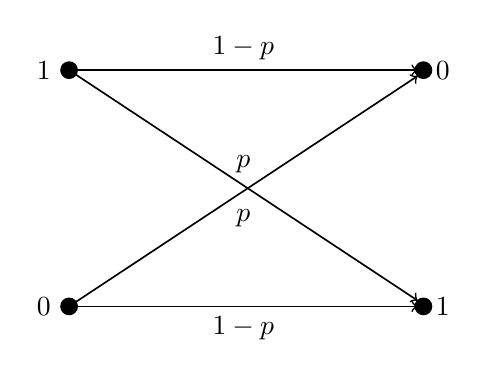
\begin{tikzpicture}
\centering
\filldraw (0,0) circle (3pt);
\filldraw (0,3) circle (3pt);
\filldraw (4.5,0) circle (3pt);
\filldraw (4.5,3) circle (3pt);
\draw[->,line width=0.6pt] (0,3) node[left=3pt] {$1$} -- node[above=1pt] {$p$} (4.425,0.075);
\draw[->,line width=0.6pt] (0,0) node[left=3pt] {$0$} -- node[below=3pt] {$p$} (4.425,2.925);
\draw[->,line width=0.6pt] (0,0) -- node[below] {$1-p$} (4.425,0.00)  node[right=3pt] {$1$};
\draw[->,line width=0.6pt] (0,3) -- node[above] {$1-p$} (4.425,3) node[right=3pt] {$0$};
\end{tikzpicture}
\caption{Binary Symmetric Channel\label{fig:bscChannel}}
\end{figure}

The purpose of the study is to quantify the effects of different parameters of the convolutional code, namely the constraint length and the code rate. In order to achieve the best performance a trade-off analysis on the parameters needs to be performed. 
All simulations are conducted by utilizing MATLAB. Section \ref{sec:methodSection} presents the approach used to systematically determine the effect of code parameters in different channels. \todo{Analysis performed in sections 2-3-4}. Finally, section \ref{sec:conclusionSection} summarizes the findings.



\section{Method}
\label{sec:methodSection}

As a starting point for the analysis, the following 3 sets of generator polynomials convolutional codes were given. The first subscript of each polynomial represents the code number for later reference, and the second subscript is the index of the generator polynomial associated with the code.

\begin{align*}
\begin{matrix}
\textbf{Code 1}&\textbf{Code 2}&\textbf{Code 3}\\
g_{1,1}(x) = 1 + x + x^2 + x^3 + x^6&g_{2,1}(x) = 1 + x^2 + x^3&g_{3,1}(x)=1 + x^2\\
g_{1,2}(x) = 1 + x^2 + x^3 + x^5 + x^6&g_{2,2}(x)=1 + x + x^3&g_{3,2} = 1+x+x^2\\
&g_{2,3}(x) = 1+x+x^2+x^3&g_{2,3}(x)=1+x+x^2\\
&&g_{3,4}(x) = 1+x+x^2
\end{matrix}
\end{align*}

The investigation is concerned with how the convolutional codes performs when random and burst errors are introduced in the channels. For this purpose, MATLAB scripts that would allow simulating transmission of a message over the given types of channels are created.
In each script, it is possible to adjust the input message length and the number of times the simulation should run. Increasing the number of simulation iterations will generate smoother lines of the figures, by averaging the results of multiple realizations. This reduces effects of the stochastic nature of the simulation. For the simulations presented in the paper, the result is from $25$ runs. 
An additional file, (\verb@trellisGenerator.m@), defines the convolutional code generator polynomials used. The code polynomials used for coding and decoding may be easily specified by modifying this file.
The following sections present the methods used for simulation.
\subsection{Binary Symmetric Channel}
The file \verb@randomErrors.m@ presents the method of simulation of random errors in a BSC. In the script, it is possible to modify the following simulation parameters:
\begin{itemize}\setlength\itemsep{0pt}
   \item \verb@maxCER@: Maximum Channel bit Error Rate (CER) that is simulated.
   \item \verb@CERLevels@: The number of different CER levels for the simulation. This value determines the granularity of the steps as the CER is increased from $0$ to \verb@maxCER@.
\end{itemize}
For the specified number of iterations, the script generates a message of the given length. The message is then encoded using the code definitions from \verb@trellisGenerator.m@ file and for each of the codes, the encoded data is altered using the different levels of CER. For a given CER, the exact amount of bits corresponding to that CER is altered, independently positioned. The alteration of bits at random positions in the message simulates the channel noise. For each of the error levels, the received codeword is then decoded and compared to the transmitted version, calculating the Bit Error Rate (BER).

\subsection{Deterministic Bursts}

The file \verb@burstErrors.m@ presents the method of simulation of deterministic burst errors. In the script, it is possible to modify the following simulation parameters:
\begin{itemize}\setlength\itemsep{0pt}
   \item \verb@BurstLevels@: The number of different error burst lengths that are introduced on the channel. Set to $n$, bursts of length $\{0, 1, \dots , n-1 \}$ are simulated.
   \item \verb@nBursts@: The total number of error bursts to be introduced on the channel.
   \item \verb@burstSep@: The number of unaffected bits between error bursts. Must be large enough that each burst does not influence adjacent bursts.
\end{itemize}
In a similar manner as in the BSC, for the specified number of iterations, the script generates a message of the given length. The message is then encoded using the code definitions from \verb@trellisGenerator.m@ file and for each of the codes, the encoded data is altered using by introducing errors in bursts of a specific length. The burst error represents a channel being temporarily affected by interference. For each burst length, the data is then decoded and compared to the transmitted version, calculating the number of message errors per burst of a specific length.
\subsection{Markov Burst Error Channels}
While the previous channels are easy to deal with in theory, in many cases it does not match the reality well. In practice, errors are neither entirely independant and random, nor deterministic bursts, but rather stochastic with correlation. Effects such as deep fades in wireless channels cause the probability of a symbol being in error to be much larger if the previous symbol was an error. This causes errors to appear in bursts. A simple model of such a channel can be created by using a two-state Markov chain, as shown on figure \ref{fig:markovChain}. For each time-step (each bit in the channel), the current state of the chain is updated and a bit is output. The transition probabilities $p_{01}$ and $p_{10}$ determines how the error pattern will behave. $p_{01}$ is the probability of starting a burst, and $p_{10}$ is the probability of ending the current burst. In this way, the length of bursts, BL, will be geometrically distributed:\todo{Can add a plot of this for chosen p10 if room for it.}
\begin{equation}
P(\text{BL} = k) = (1-p_{10})^{k-1}  p_{10}
\end{equation}
meaning that smaller bursts are more likely than long bursts. The Markov burst error channel will be simulated by basing the error pattern on this Markov chain.
\begin{figure}
\centering
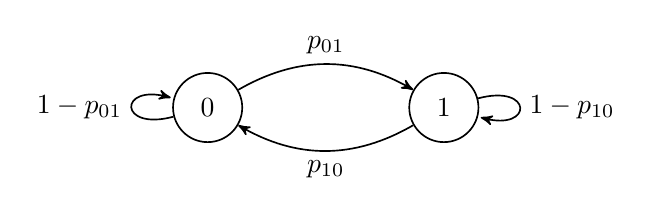
\begin{tikzpicture}[->, >=stealth', auto, semithick, node distance=3cm]
\centering
\node[state] (A) at (0,0) {$0$};
\node[state] (D) at (3,0) {$1$};
\path(A) edge[loop left] node{$1-p_{01}$} (A);
\path(A) edge[bend left] node{$p_{01}$} (D);
\path(D) edge[bend left] node{$p_{10}$} (A);
\path(D) edge[loop right] node{$1-p_{10}$} (D);
\end{tikzpicture}
\caption{Markov Chain for Burst Channel Simulation.}
\end{figure}

The file \verb@markovErrors.m@ contains the implementation of this method for simulation of these random burst errors. It is possible to modify the following simulation parameters:
\begin{itemize}\setlength\itemsep{0pt}
\item \verb@burstProbabilityMax@, max value for $p_{01}$ to be simulated.
\item \verb@burstProbabilityLevels@, number of different levels of $p_{01}$ to be simulated. Determines the granularity of the simulation.
\item \verb@p10@, the transition probability from state $1$ to $0$
\end{itemize}
For each of the specified number of simulations, a message is generated and encoded using the code definitions from \verb@trellisGenerator.m@ and for each of these transmission through a number of Markov channels, where the transition parameter $p_{01}$ is varied according to the specified parameters, is simulated. The CER of each Markov channel is calculated. The received codeword is then decoded and compared to the real message. Finally, the BER is calculated.

\subsection{Additional Codes}
The results for the given codes are presented in section \ref{sec:givenCodesSection}. While it is possible to compare the codes, it is not entirely fair to compare codes with both varying code rate and constraint length. It is more reasonable to compare the performance of codes with the same code rate or same constraint length, to show the effect of changing only one of the parameters.



\todo{R: Changed this --- Even though the results, show as expected, a negative relation between the code rate and constraint length on one side and error rates on the other, we considered that simulations where we are varying only one of the factors are necessary. This approach allows us not only to confirm that both the factors influence the error correction capabilities of the code, but also to assess their sensibility.}

In order to do so, additional codes must be introduced for comparison. These codes are presented as Code 4 to 9, and specified by the generator polynomials below:

\begin{align*}
\begin{matrix}
\textbf{Code 4}&\textbf{Code 5}&\textbf{Code 6}\\
g_{4,1}(x) = 1 + x^2 + x^3&g_{5,1}(x) = 1 + x^2&g_{6,1}(x)=1 + x + x^2 + x^3 + x^6\\
g_{4,2}(x) = 1+x+x^2+x^3&g_{5,2}(x) = 1+x+x^2&g_{6,2}(x)=1 + x^2 + x^3 + x^5 + x^6\\
&&g_{6,3}(x)=1 + x + x^2 + x^3 + x^4 + x^5 + x^6\\
\end{matrix}\\
\begin{matrix}
\textbf{Code 7}&\textbf{Code 8}&\textbf{Code 9}\\
g_{7,1}(x) = 1 + x^2&g_{8,1}(x) = 1 + x + x^2 + x^3 + x^6&g_{9,1}(x)=1 + x^2 + x^3\\
g_{7,2}(x) = 1+x+x^2&g_{8,2}(x) = 1 + x + x^3 + x^4 + x^6&g_{9,2}(x)=1 + x + x^3\\
g_{7,3}(x) = 1+x+x^2&g_{8,3}(x) = 1 + x^2 + x^3 + x^5 + x^6&g_{9,3}(x)=1+x+x^2+x^3\\
&g_{8,4}(x) = 1 + x + x^2 + x^3 + x^4 + x^5 + x^6&g_{9,4}(x)=1+x+x^2+x^3\\
\end{matrix}
\end{align*}
These codes can be grouped with the given codes by code rate and by constraint length, as follows:
\begin{table}[h]
\centering
\begin{tabular}{ll}
\hline
Code rate &  Codes \\ \hline
1/2 & Code 1, Code 4, Code 5 \\
1/3 & Code 2, Code 6, Code 7 \\
1/4 & Code 3, Code 8, Code 9 \\
\end{tabular}
\caption{Grouping of codes based on code rate}
\end{table}

\begin{table}[h]
\centering
\begin{tabular}{ll}
\hline
Constraint length &  Codes \\ \hline
3 & Code 3, Code 5, Code 7 \\
4 & Code 2, Code 4, Code 9 \\
7 & Code 1, Code 6, Code 8 \\
\end{tabular}
\caption{Grouping of codes based on constraint length}
\end{table}

All of these groups can be chosen for simulation in \verb@trellisGenerator.m@. The results obtained for the constant code rate of 1/2 and variable constraint length are presented in section \ref{sec:constantCodeRateSection}. Similarly, the results obtained by having a constant constraint length of 4 and variable code lengths are presented in section \ref{sec:constantContraintLengthSection}.
\section{Given codes}
\label{sec:givenCodesSection}	
 
The results obtained for the initially given code polynomials are presented in this section. By examining the result for the BSC on figure \ref{fig:givenRandomFigure}, it can be seen that the code with the highest code rate performs best. This is expected, since more redundancy is added. The constraint length does not appear to have a major influence on the performance in this channel, but it is hard to conclude anything when varying multiple parameters at once. Therefore, codes with fixed constraint length are compared in section \ref{sec:constantContraintLengthSection}.
For the burst simulations, it is seen in figure \ref{fig:givenBurstFigure} that Code 1 on average has significantly more errors in the message than the two other codes when comparing at the same burst length.
The result for the MBEC is more interesting. Here, the winner is less clear, and Code 1 and Code 2 perform equally well at low CER, while Code 2 performs best higher values. However, the code rate of Code 1 is only $1/2$ in contrast to the code rate of $1/3$ for Code 2, so it seems that the constraint length do have a big influence in this channel. This is investigated further in section  \ref{sec:constantCodeRateSection}.

\begin{figure}
\centering
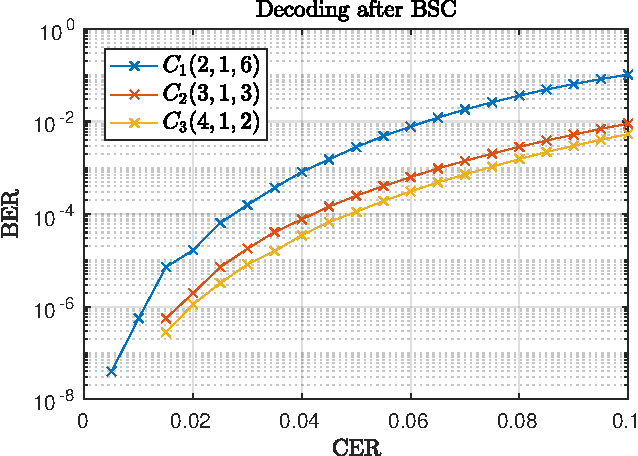
\includegraphics[scale=1]{../figures/qirandom.pdf} 
\caption{\textit{Comparison of given codes in BSC}\label{fig:givenRandomFigure}}
\end{figure}

\begin{figure}
\centering
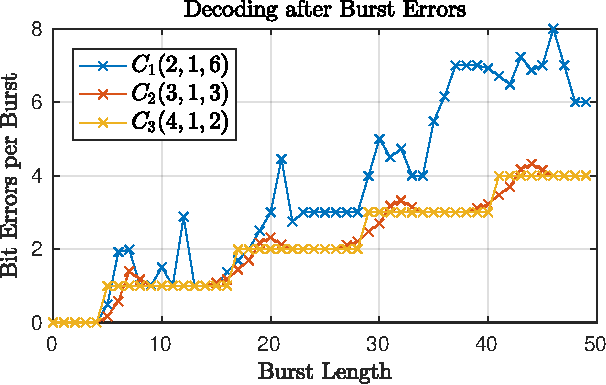
\includegraphics[scale=1]{../figures/qiburst.pdf} 
\caption{\textit{Comparison of given codes burst correction capabilities}\label{fig:givenBurstFigure}}
\end{figure}

\begin{figure}
\centering
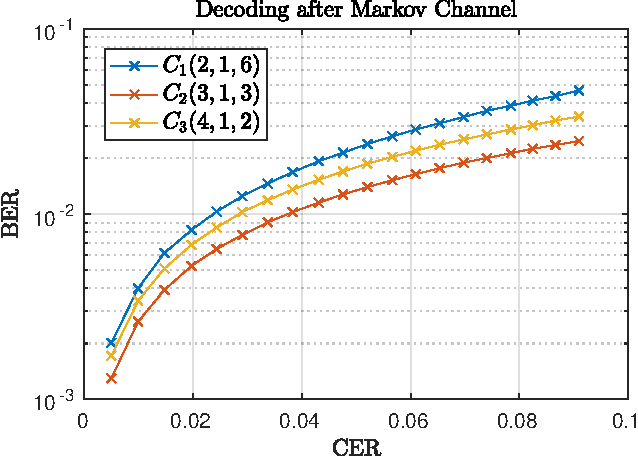
\includegraphics[scale=1]{../figures/qimarkov.pdf} 
\caption{\textit{Comparison of given codes in MBEC}\label{fig:givenMarkovFigure}}
\end{figure}

\section{Constant code rate\label{sec:constantCodeRateSection}}
This section presents the results obtained by coding the messages with codes having the same code rate (in our case 1/2) but different constraint lengths. Figure \ref{fig:constantCodeRateRandomFigure} indicates that having a higher constraint length reduced the number of decoded errors. However, this is true only for relatively small channel error rates. It can be seen in figure \ref{fig:constantCodeRateRandomFigure} that for our examples, the code with the highest constraint length starts to perform worse than the other at a channel error rate close to 0.08. 
The results of the simulation performed using a channel that introduces bursts errors are shown in figures \ref{fig:constantCodeRateBurstFigure} and \ref{fig:constantCodeRateMarkovFigure}. \todo{Continue here}


\begin{figure}
\centering
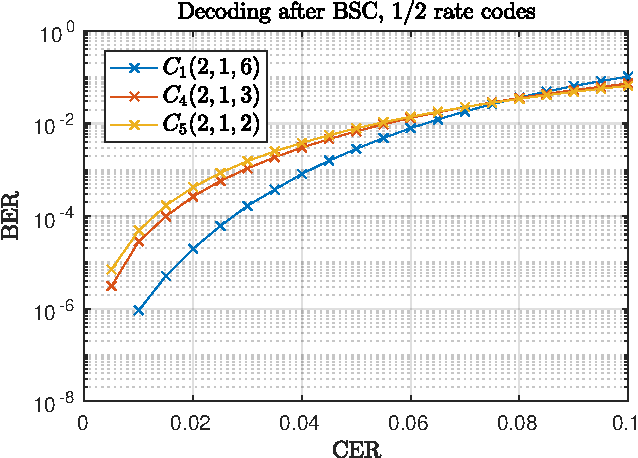
\includegraphics[scale=1]{../figures/extra12rand.pdf} 
\caption{1/2 rate\todo[inline]{change caption}\label{fig:constantCodeRateRandomFigure}}
\end{figure}

\begin{figure}
\centering
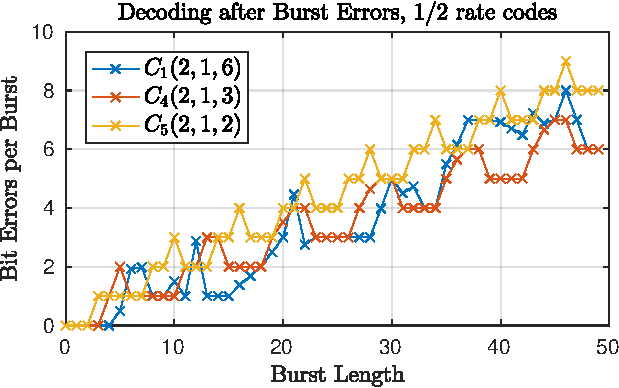
\includegraphics[scale=1]{../figures/extra12burst.pdf} 
\caption{1/2 rate\todo[inline]{change caption}\label{fig:constantCodeRateBurstFigure}}
\end{figure}

\begin{figure}
\centering
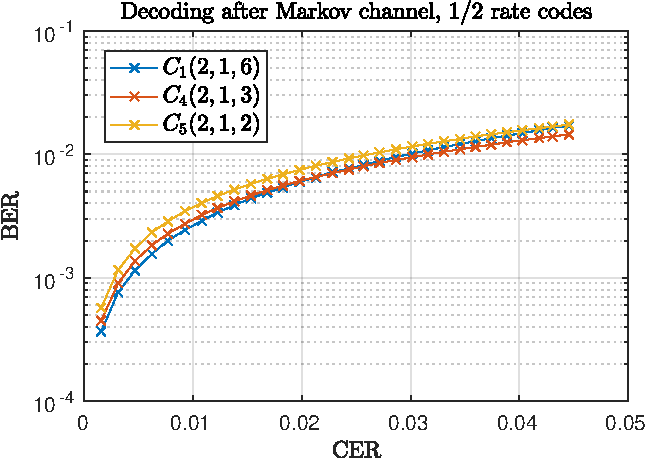
\includegraphics[scale=1]{../figures/extra12markov.pdf} 
\caption{1/2 rate\todo[inline]{change caption}\label{fig:constantCodeRateMarkovFigure}}
\end{figure}
\section{Constant constraint length\label{sec:constantContraintLengthSection}}
In this section, the effect of the code rate is investigated by fixing the constraint length. It has been chosen to fix the constraint length at $4$, and use codes with code rate $1/2$, $1/3$, and $1/4$, i.e. Code 4, Code 2 and Code 9, as specified in table \ref{tab:constraintLength}.
\\[6pt]
Figure \ref{fig:constantContraintRandomFigure} indicates that increasing the code rate greatly reduces the amount of errors in the BSC, as expected. Decreasing the code rate from $1/2$ to $1/3$ or from $1/3$ to $1/4$ reduces the BER by approximately an order of magnitude.
The effect on burst errors is also clear, as seen on figure \ref{fig:constantContraintBurstFigure}. Decreasing the code rate makes each burst cause less errors in the message. The same is seen in the MBEC, as shown on figure \ref{fig:constantContraintMarkovFigure}. The decrease of BER in this channel is much smaller than in the BSC, however.
In conclusion, the effect of varying the code rate is straightforward. More redundancy is added in the codeword causes less bit errors in the message, of course at the cost of decreasing the throughput in the channel.





%
%This section presents the results obtained by coding the messages with codes having the same constraint length (in our case, 4) but different code rates. All the three figures (figures \ref{fig:constantContraintRandomFigure}, \ref{fig:constantContraintRandomFigure}, \ref{fig:constantContraintMarkovFigure}) show the same result - the error correction capabilities are better when the code rate is lower. This is due to the fact that more redundancy is added to each message. As opposed to varying the constraint length, the variations in code rate have a straight forward result.

\begin{figure}
\centering
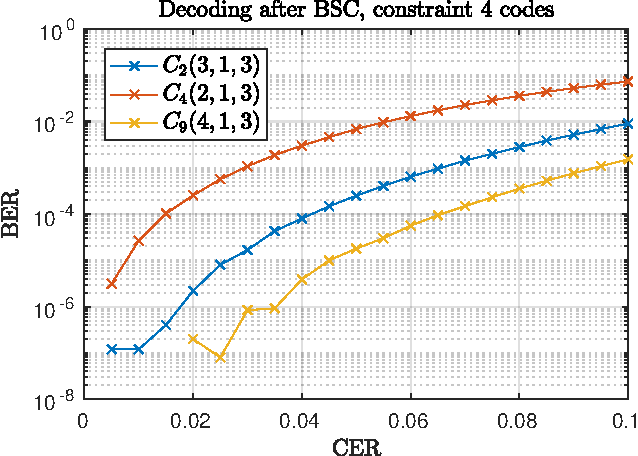
\includegraphics[scale=1]{../figures/const4rand.pdf} 
\caption{\textit{Comparison of codes with constraint length 4 and varying code rates in BSC}\label{fig:constantContraintRandomFigure}}
\end{figure}

\begin{figure}
\centering
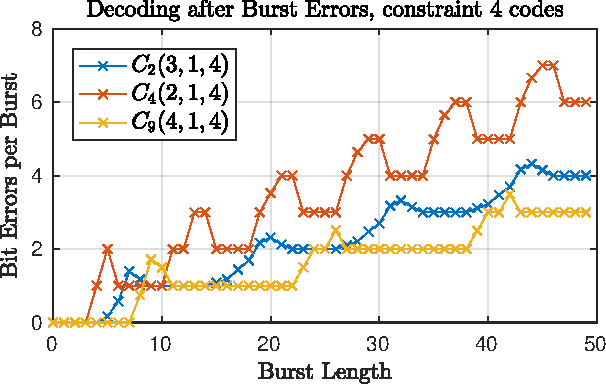
\includegraphics[scale=1]{../figures/const4burst.pdf} 
\caption{\textit{Comparison of codes with constraint length 4 and varying code rates burst correction capabilities}\label{fig:constantContraintBurstFigure}}	
\end{figure}

\begin{figure}
\centering
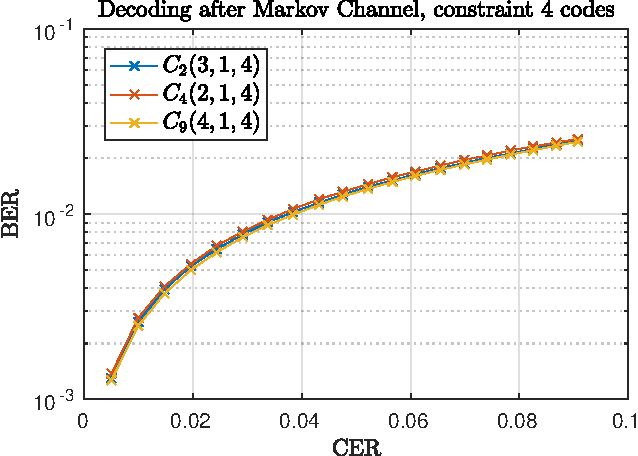
\includegraphics[scale=1]{../figures/const4markov.pdf} 
\caption{\textit{Comparison of codes with constraint length 4 and varying code rates in MBEC}\label{fig:constantContraintMarkovFigure}}
\end{figure}
\todo[inline] {Compare different codes with the same constraint length and different code rate (more generator polynomials).}

\section{Conclusion}
\label{sec:conclusionSection}



 




\end{document}